% Copyright (c) 2020 Carl Martin Ludvig Sinander.

% This program is free software: you can redistribute it and/or modify
% it under the terms of the GNU General Public License as published by
% the Free Software Foundation, either version 3 of the License, or
% (at your option) any later version.

% This program is distributed in the hope that it will be useful,
% but WITHOUT ANY WARRANTY; without even the implied warranty of
% MERCHANTABILITY or FITNESS FOR A PARTICULAR PURPOSE. See the
% GNU General Public License for more details.

% You should have received a copy of the GNU General Public License
% along with this program. If not, see <https://www.gnu.org/licenses/>.

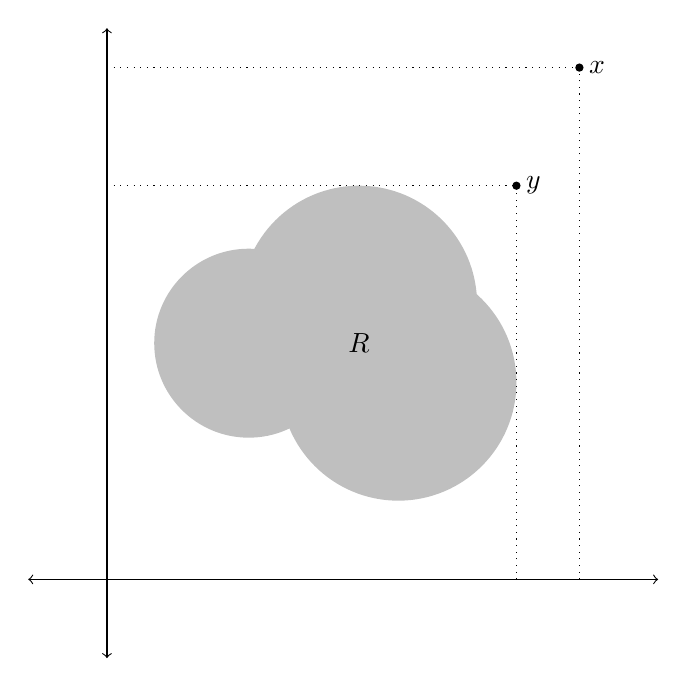
\begin{tikzpicture}[scale=1]
	
	% blob
	\fill[lightgray] (3.2,3.5) circle[radius=1.5cm];
	\fill[lightgray] (3.7,2.5) circle[radius=1.5cm];
	\fill[lightgray] (1.8,3) circle[radius=1.2cm];
	\draw (3.2,3) node {$R$} ;

	% \widebar{a}
	\draw (6,6.5) node[anchor=west] {$x$} ;
	\fill (6,6.5) circle[radius=1.5pt];
	\draw[dotted] (6,0) -- (6,6.5);
	\draw[dotted] (0,6.5) -- (6,6.5);

	% a^*
	\draw (5.2,5) node[anchor=west] {$y$} ;
	\fill (5.2,5) circle[radius=1.5pt];
	\draw[dotted] (5.2,0) -- (5.2,5);
	\draw[dotted] (0,5) -- (5.2,5);

	% axes
	\draw[<->] (-1,0) -- (7,0);
	\draw[<->] (0,-1) -- (0,7);

\end{tikzpicture}